%!TEX root = ../bachelorthesis.tex

\pagenumbering{arabic}
\setcounter{page}{1}

\chapter{Einleitung}
\markboth{Einleitung}{}
\label{sec:Einleitung}
\section{Kontext}
Im Rahmen des Studiums der Sozialinformatik wurde in der \ac{kita} \textit{Schloss Ardeck} in Gau-Algesheim vom Autor dieser Arbeit ein lokales soziales Netzwerk als Kommunikations- und Dokumentenmanagementsystem eingeführt. In dem \textit{KitaNet} genannten System können durch die Leitung und Mitarbeitenden der Einrichtung beispielsweise Elternbriefe ausgetauscht und erarbeitet werden oder Terminabsprachen und Diskussionen geführt werden, auch wenn die Kolleginnen aufgrund von Schichtdiensten nicht immer direkten Kontakt haben. \\ Das Projekt wurde innerhalb von zwei Jahren realisiert und in der \ac{kita} implementiert.

Technisch besteht KitaNet aus einer \ac{vm} auf einem NAS-System der Firma QNAP. Auf der \ac{vm} läuft die auf der Skriptsprache \ac{php} basierende Software \textit{HumHub}. Diese arbeitet mit einer durch QNAP bereitgestellten Variante eines \ac{ldap}-Servers zur Benutzerverwaltung zusammen. Dies war notwendig, um der Leitung der Kita eine Möglichkeit zu bieten, Nutzerpasswörter grundzustellen und neue Nutzer anzulegen. Gerade das Grundstellen von Passwörtern ist in der täglichen Arbeit leider häufiger notwendig, als von den Projektdurchführenden geplant und bindet somit einen nicht unerheblichen Teil der Arbeitszeit der Leitung.

HumHub selbst bietet die Möglichkeit, beim Nutzer eine E-Mail-Adresse zu hinterlegen, über die dann ein Grundstellen des Passwortes möglich ist. Hierfür wäre allerdings ein E-Mail-Server innerhalb des Netzwerkes notwendig, da das Gesamtsystem KitaNet aus Datenschutzgründen keine direkt eVerbindung zum Internet hat. Die Funktion zum zurücksetzen des Passworts wurde im Rahmen des IT-Projektes nicht genutzt. Im Rahmen dieser Bachelorarbeit wird nun der Frage nachgegangen werden, wie die Implementierung eines Mailservers in die Umgebung aus \ac{vm}, \ac{ldap} und HumHub durchgeführt werden kann. Hierfür wird die in der \ac{kita} vorliegende Umgebung auf einem separaten Server nachgestellt werden, um den Produktivbetrieb in der \ac{kita} nicht zu gefährden.

\section{Aufbau und Gestaltung der Arbeit}

In dieser Bachelor-Thesis wird zunächst KitaNet sowie die hier vorliegende Hardwareumgebung und das Einsatzszenario erläutert werden. Hier werden auch Hinderungsgründe genannt, die eine Umsetzung der in dieser Thesis beschriebenen Lösung in den Produktivbetrieb der Kita verhindern. In diesem Kapitel wird auch die Funktionalität eines \ac{ldap} beschrieben.

Das nächste Kapitel behandelt zunächst die Funktionsweise eines \ac{smtp}-Servers. Im Anschluss werden die Anforderungen und Nutzungsszenarien des Mailservers für KitaNet festgelegt. Die Anforderungen umfassen dabei zum Einen Punkte wie die Zusammenarbeit mit einem Nutzerverzeichnis, verbunden mit einer möglichen Automation des Anlegens von Mail-Nutzern, werden aber zum Anderen auch nichtfunktionale Aspekte, wie den zu erwartenden Pflegeaufwand oder die finanzielle Belastung durch etwaige Lizenzkosten, beachten. \textbf{Hinweis auf RE einarbeiten!}

Die benannten Nutzungsszenarien bilden die Grundlage zur Formulierung von Tests, die die Funktionalität und Praxistauglichkeit der späteren Installation sicherstellen werden. Die Beschreibung dieser Tests bildet den Abschluss  dieses Kapitels.

Anschließend werden die zur Wahl stehenden Softwarepakete \textit{postfix} und \textit{Exim} vorgestellt. Die im vorherigen Kapitel formulierten Anforderungen werden mit dem Funktionsumfang der Softwarepakete abgeglichen. Aufgrund der Ergebnisse dieses Abgleichs erfolgt die Entscheidung. 

Dessen Installation bildet das nächste Kapitel. Es wird dargestellt, ob und welche Anpassungen durchzuführen sind, um den \ac{smtp}-Server in die vorliegende Umgebung zu integrieren. Auch die Anbindung an das \ac{ldap} wird beschrieben.
Die Dokumentation der durchgeführten Tests schließt das Kapitel ab. An dieser Stelle soll auch kritisch hinterfragt werden, ob die im Vorfeld formulierten Tests ausreichend spezifisch waren oder Anpassungen an diesen vorzunehmen waren.

Ein persönliches Fazit schließt diese Bachelor-Thesis ab.

\textit{Erstmalige Fachbegriffe oder Eigennamen} werden \textit{kursiv} dargestellt und in diesem Kontext erläutert.  \\ \textquote{Zitate werden mit französischen Anführungszeichen gekennzeichnet}. \\ \verb+Code oder ähnliches+ wiederum werden immer in einer \verb+Monospace-Schriftart+ ausgegeben, um ihn vom umliegenden Text zu separieren. \\ Abkürzungen und Akronyme wie \zb \ac{nas} werden bei der ersten Erwähnung kursiv ausgeschrieben und mit der Abkürzung benannt. Diese findet sich dann auch im Abkürzungsverzeichnis. Im weiteren Text erscheinen Sie nur noch abgekürzt. 

\section{Methodik}

Wie im vorherigen Abschnitt beschrieben, erfolgt die Auswahl der zu installierenden Software aufgrund des Abgleichs mit zuvor festgelegten Anforderungen.

Hierzu werden die Angaben des jeweiligen Herstellers, respektive bei nicht kommerzieller Software der Projektverantwortlichen, herangezogen um eine objektive Vergleichbarkeit der Softwareprodukte sicherzustellen. Die Entscheidung wird somit grundsätzlich aufgrund objektiver Grundlagen getroffen.  Da beispielsweise die finanzielle Situation der \ac{kita} nur einen geringen Spielraum für Investitionen zulässt, können die formulierten Anforderungen nicht vollständig gleichwertig behandelt werden. Werden Anforderungen, \zb aufgrund wirtschaftlicher Erwägungen, unterschiedlich gewichtet, wird dies gesondert im Text erwähnt.

Es findet somit eine Mischung aus qualitativer und quantitativer Forschung statt.

Die Implementierung erfolgt anschließend im Rahmen eines Experiments in einer KitaNet nachempfunden Umgebung.

Die Funktionsweise von KitaNet und sein Nutzen für die \ac{kita} werden nun im nächsten Kapitel erläutert.

\chapter{KitaNet}
\markboth{KitaNet}{}
\label{sec:KitaNet}
%Kurze Beschreibung von technischer Basis von KitaNet. Was sind soziale Netzwerke?
%Ablauf beim Grundstellen von Passwörtern wird erläutert.

KitaNet ist der Arbeitstitel eines IT-Projektes, das im Rahmen des Studiums der Sozialinformatik vom Autor dieser Thesis mit einem Kommilitonen durchgeführt wurde. Hierfür wurde in Zusammenarbeit mit der \ac{kita} Schloss Ardeck in Gau-Algesheim ein soziales Netzwerk installiert, über welches die Bediensteten der Kita eine Plattform zum Austausch und zur Kommunikation erhalten. 

Die \ac{kita} betreut ca. 170 Kinder im Alter von einem bis sechs Jahren. Hierfür beschäftigt sie 30 pädagogische Fachkräfte, welche die ihnen anvertrauten Kinder in acht Gruppen betreuen. Die Kita befindet sich in kommunaler Trägerschaft \citep[vgl.][]{kitaweb}.

Für die Umsetzung der Idee eines sozialen Netzwerkes konnten die Studenten unter anderem von dem Umstand profitieren, dass jede Gruppe der Kita mit Notebooks ausgestattet ist, über welche die Kinder Lernspiele spielen, aber auch unter Betreuung der Erzieher erste Erfahrungen mit dem Internet sammeln.

Die technische Umgebung in der Kita, sowie die Umsetzung des sozialen Netzwerks werden nun genauer beschrieben. Auch werden hier Unterschiede zur Testumgebung dieser Bachelor-Arbeit aufgezeigt.

\section{Hardware}
%Beschreibt den technischen Aufbau von KitaNet in der Kita selbst.
%Abweichungen vom Aufbau für Studienprojekt werden erläutert. Was weicht ab?
%Verhindert die für dieses Bachelorarbeit eingesetzte Hardware eine Umsetzung in der Kita?
In der \ac{kita} wurde im Rahmen einer Elterninitiative ein lokales Netzwerk bestehend aus fünf WLAN-Routern installiert. Dieses \ac{lan} vernetzt nicht nur die vier Gebäudeteile der Kita miteinander, es stellt zugleich die telefonische Erreichbarkeit der einzelnen Gruppen sicher. Dieses Netzwerk wurde in der Vergangenheit unter anderem dazu genutzt, Dokumente am zentralen Netzwerkdrucker im Büro der Leitung auszudrucken.

Die Studierenden entschieden sich zur Umsetzung des Projektes KitaNet für die im Anschluss näher erläuterte Software HumHub.
Einer der Vorteile war, dass diese kostenlos auf einem privaten Server installiert werden konnte. Die Installation erfolgte auf einem \ac{nas} der Firma \textit{QNAP}, genauer einem QNAP TS-253B \citep[vgl.][]{qnap}. Im von der Verwaltungssoftware des \ac{nas} bereitgestellten \textit{VM-Manager} wurde ein virtueller Ubuntu-Server erstellt, auf dem die Software Humhub installiert wurde.

Im Vergleich zum Produktivaufbau ergibt sich hier der erste Unterschied zum Versuchsaufbau für diese Arbeit. Anstatt einen Ubuntu-Server als virtuelle Maschine in einem \ac{nas} aufzusetzen, wird hier der Server auf echter Hardware betrieben. 

Die Nutzung einer \ac{vm} im Rahmen des Projektes war damit begründet, dass die Softwareinstallation auf dem NAS selbst nur in einem engen Rahmen möglich war. Die Nutzung einer Ubuntu-VM ermöglichte es den Studenten, die Installation in einer standardisierten Umgebung vornehmen zu können, ohne etwaige Besonderheiten des QNAP-Betriebssystems berücksichtigen zu müssen.

Im Rahmen dieser Bachelorarbeit wird, wie eingangs beschrieben, die Produktivumgebung bestmöglich nachgebildet. Hierfür dient ein Fujitsu Esprimo C5730 E als Hardware, auf der Ubuntu 20.04 LTS als Betriebssystem installiert wurde. Nach Ansicht des Autors hat die verwendete Hardware keine nennenswerte Auswirkung auf die Funktionalität des beschriebenen Versuchsaufbaus. \\ Einzige zu beachtende Besonderheit ist, dass das später beschriebene \ac{ldap} in der Produktivumgebung nicht auf der \ac{vm} sondern auf dem \ac{nas} selbst ausgeführt wird. Hier ist dann die Konfiguration für eine Übernahme ins Produktivsystem entsprechend anzupassen.

Wie bereits erwähnt, kommt innerhalb der \ac{vm} die Software HumHub zum Einsatz. Der Umfang und die Funktionen dieser Software wird nun kurz erläutert.

\section{HumHub}

Bei ihren Recherchen für die Umsetzung des IT-Projektes stießen die Studenten auf die Social-Network-Software HumHub. Die Software ist quelloffen und wird von der HumHub GmbH \& Co.KG aus München vertrieben. Die Möglichkeit, die Software kostenlos für nicht kommerzielle Zwecke installieren und betreiben zu können, gab letztlich den Ausschlag für Entscheidung  \textquote{HumHub ist eine freie und sehr flexible Social Networking Software, die auf eigenen Servern gehosted werden kann} \citep{humhubmain}.

Die Grundfunktionen von HumHub und die Möglichkeit der Erweiterung der Grundfunktionen soll im Weiteren betrachtet werden.

\subsection{Spaces}

Spaces geben HumHub seine Grundstruktur. \textquote{A space serves as an independent area within your network with an own set of members, permissions, settings and modules} \citep{spaces}. 
Eine Nutzerin kann Mitglied mehrerer Spaces sein und innerhalb der Spaces verschiedene Rollen einnehmen. Diese reichen von \textit{Besitzer} des Spaces, der nahezu volle Kontrolle über sämtliche Nutzer und Beiträge innerhalb des jeweiligen Spaces hat, über den \textit{Moderator}, der Beiträge verwalten kann, bis hin zum normalen Mitglied, das Beiträge erstellen kann, wenn dies vom Besitzer erlaubt wurde.  

Zentraler Sammelpunkt für Beiträge ist der \textit{Stream}, dessen Inhalt sich je nach Kontext verändert. Betrachtet ein Nutzer seine Startseite, werden ihm sämtliche Beiträge aus all seinen Spaces angezeigt. Befindet er sich in einem Space, sind nur dort erstellte Beiträge sichtbar.

Mit den Spaces bietet Humhub die Möglichkeit, Gruppenstrukturen abzubilden. Jedoch kann in den Gruppen nicht viel mehr getan werden, als Bilder oder Texte zu erstellen und diese zu kommentieren.
Sein volles Potential kann Humhub mit den Möglichkeiten entfalten, \textit{Module} zur Funktionserweiterung nachzuladen.

\subsection{Module}

\textquote{The feature set of your HumHub network can be extended by installing additional modules} \citep[][]{modules}. Zur Erweiterung der Funktionalität stehen diverse Module wie Kalender, Dateiablage, Abstimmungen oder ein Wiki zur Verfügung.
Module können für einzelne Spaces aktiviert werden, um den Bedürfnissen des jeweiligen Kontext gerecht zu werden \citep[vgl.][ff.]{modules}. Ein Space, der zur Organisation des Sommerfestes der Kita eingerichtet wurde, benötigt \zb in der Regel keinen Kalender, sehr wohl aber eine Dateiablagestruktur.
So wird der einzelne Space nicht mit unnötigen Features überladen, die vom Zweck der Umgebung ablenken würden. 

Die Module werden zum Teil von HumHub selbst bereit gestellt, es besteht jedoch auch die Möglichkeit für Entwickler, eigene Erweiterungen zu schreiben.

Besondere Erwähnung sollte die Erweiterung \textit{Ankündigungen} erhalten. 
Eine Ankündigung wird im Stream des Spaces grundsätzlich wie eine einfache Mitteilung (ein \textit{Post}) angezeigt. Einzige Besonderheit ist, dass die Nutzer diesen Post mit einem Klick zur Kenntnis nehmen können. Diese Kenntnisnahme kann dann vom Ersteller des Beitrags oder einem Moderator \zb als Excel-Datei exportiert werden  \citep[Quellcode unter][]{announcement}. Da dieser Mitteilung auch Dateien angehängt werden können, konnten die Studenten die Forderung der Leitung nach Protokollierung der Einsichtnahme von Dokumenten Rechnung tragen.


\section{OpenLDAP}

Zum Anlegen der Benutzer innerhalb des KitaNet wurde die Benutzerverwaltung des QNAP-NAS auf Basis von \textit{OpenLDAP} genutzt. Die Funktionsweise von OpenLDAP wird daher ebenfalls kurz erläutert.

\subsection{Funktionsweise und Datenmodell}

\ac{ldap} beschreibt  ein Protokoll, welches die zentrale Ressourcenverwaltung innerhalb eines Netzwerkes über eine Datenbank abwickelt.
\textquote{Verzeichnisdienste wie \textquote{OpenLDAP} ermöglichen es Ihnen, die Verwaltung der Ressourcen zentral zu steuern und an mehreren Stellen zu replizieren} \citep[][611]{Deimeke2019}. OpenLDAP stelle eine quelloffene Implementation dieses Standards nach \ac{rfc}4519 dar.

Die Ressourcen innerhalb des \ac{ldap}-Kontextes stellen sowohl Nutzer als auch Geräte dar. Das \ac{ldap} bildet ihre Attribute, wie Namen oder Gruppenzugehörigkeiten, aber auch ihre Beziehung zu- und untereinander dar. Dies wird im weiteren noch näher erläutert. 
\ac{ldap} besteht aus einer Datenbank, beinhaltet aber zugleich auch ein passendes Netzwerkprotokoll, um mit der Datenbank interagieren zu können \citep[vgl.][3]{Gietz}.

Deimeke \ua führen weiter aus, dass der Vorteil des Einsatzes eines \ac{ldap} darin besteht, dass jeder Nutzer nur noch ein Konto besitzt, dessen Passwort dann zentral verwaltet und geändert werden kann. \textquote{Um diese zentrale Verwaltung der Ressourcen realisieren zu können, wurde das \textit{Lightweight Directory Access Protocol} (LDAP) entwickelt} \citep[][611]{Deimeke2019}.

Dienste auf dem Server können auf OpenLDAP zugreifen, und die Login-Informationen und Berechtigungen für die hinterlegten Nutzer auslesen.

Innerhalb des \ac{ldap} werden die Daten zu den einzelnen Ressourcen innerhalb einer Hierarchie, dem \ac{dit} abgelegt \citep[vgl.][7]{rfc4512}. Zentraler Inhalt des \ac{dit} bilden Objekte. Diese sind die zu verwaltenden Ressourcen \citep[vgl.][614]{Deimeke2019}. 
\textquote{Ein Objekt kann sowohl ein Container sein, in dem weitere Objekte verwaltet werden, als auch ein Benutzer oder eine Gruppe sein. Eines ist bei allen Objekten aber immer gleich: Alle Objekte haben Eigenschaften, die \textit{Attribute}} \citep[][614]{Deimeke2019}. 

Eines dieser Attribute ist \zb die \textit{mail}, welche den e-Mail-Adresse des Nutzers repräsentiert \citep[][18]{rfc4519}.
\textquote{Um die Wiederverwendbarkeit von Attributen in verschiedenen Objektklassen zu ermöglichen, werden Attribute getrennt von Objekten verwaltet, und zwar in Form von Attributtypen} \citep[][615]{Deimeke2019}.

Innerhalb der Baumstruktur des \ac{dit} bilden die Nutzer die Blätter. Davon abgegrenzt werden die Äste. Diese werden von Containerobjekten gebildet, welche man auch als \ac{ou} bezeichnet \citep[vgl.][614]{Deimeke2019}.

Angesprochen werden diese Objekte über seinen \ac{dn}, einen für jedes Objekt eindeutigen Namen, vergleichbar mit dem in Dateisystemen geläufigen Prinzip von Dateipfad und Dateinamen (\zb \verb+C:/Ordner/Datei.txt+) \citep[vgl.][613]{Deimeke2019}. 

Die Mitgliedschaft der Blatt-Objekte in Gruppen kann über Suchanfragen an \ac{ldap} ausgelesen werden. Beispielsweise gibt die Suchanfrage\\ \verb+ldapsearch -x  "(mail=administrator@kitanet.local)"+ in der Konsole eines Servers den Eintrag der \ac{ldap}-Datenbank zurück, der den Mail-Adresse \textit{administrator@kitanet.local} besitzt (vgl. \autoref{ldapabfrage}).

Wie HumHub \bzw KitaNet nun mit dem \ac{ldap} zusammenarbeiten, wird im nächsten Abschnitt an ausgewählten Beispielen erläutert.

\subsection{LDAP und HumHub}

Innerhalb von HumHub kann die \ac{ldap}-Anbindung über das Webinterface konfiguriert werden \citep[vgl.][]{humldap}. Die nachfolgenden Abbildungen zeigen die Eingaben in der Testumgebung. 

\begin{figure}[H]
  \centering
  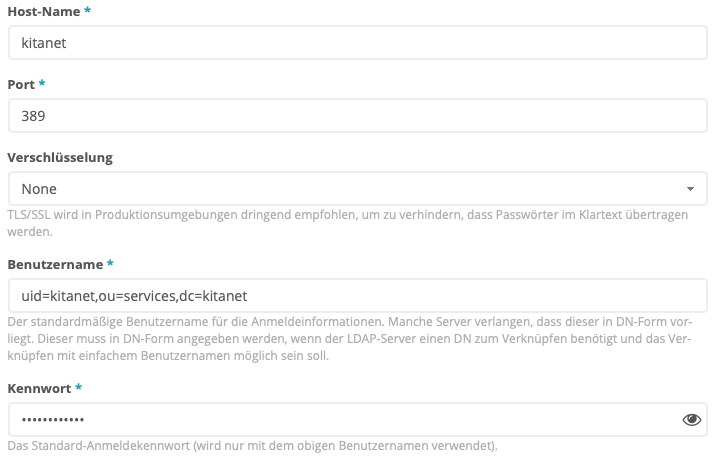
\includegraphics[width=0.9\textwidth]{res/ldapkitanet1.png}
  \caption{Teil 1 der LDAP-Konfiguration für Kitanet (Eigene Abbildung)}
  \label{fig:LDAP Kitanet Teil 1}
\end{figure}

In der Zeile \textit{Benutzername} ist ein Beispiel für eine \ac{dn} zu sehen. Für den Login im LDAP wird der Nutzer mit dem Attribut \textit{uid} \textit{kitanet}, Mitglied in der \ac{ou} \textit{services} in dem \ac{dc} \textit{kitanet} verwendet.

\begin{figure}[H]
  \centering
  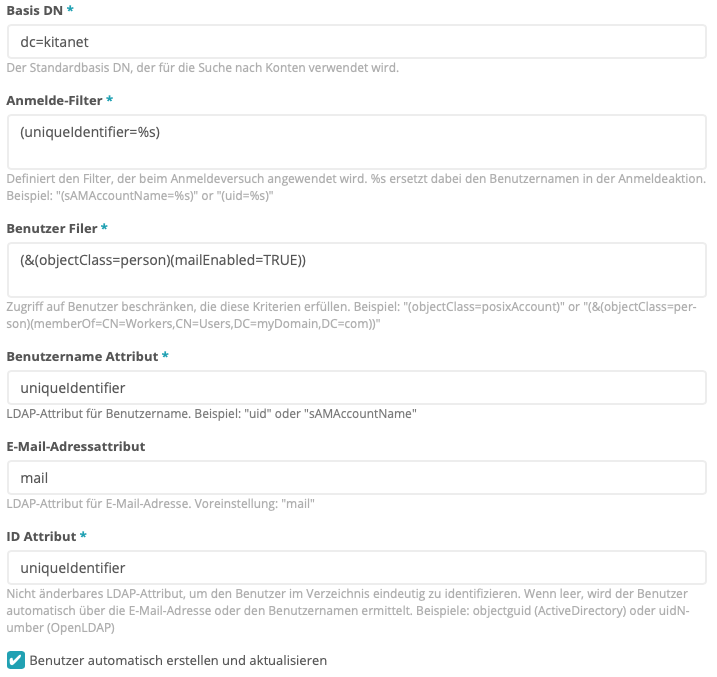
\includegraphics[width=0.9\textwidth]{res/ldapkitanet2.png}
  \caption{Teil 2 der LDAP-Konfiguration für Kitanet (Eigene Abbildung)}
  \label{fig:LDAP Kitanet Teil 2}
\end{figure}

Im unteren Teil der Einstellungen wird zunächst der \textit{Basis DN} festgelegt. Dieser legt fest in welchem Pfad des LDAP nach neuen Nutzern gesucht werden soll. Im hier vorliegenden Fall werden zunächst alle Objekte erfasst werden, sie sich in der \ac{dn} \textit{kitanet} befinden.

Der \textit{Anmelde-Filter} legt fest, welches Attribut gegen den beim Login eingegebenen Nutzernamen geprüft wird. Dies steht auch in direkter Verbindung zu den Feldern \textit{Benutzernamen Attribut} und \textit{ID Attribut} die auch beide aus dem Attribut \textit{uniqueIdentifier} ihre Informationen beziehen. 

Das Feld \textit{Benutzer Filer} legt fest, dass nur solche Objekte in Kitanet erfasst werden die ein Attribut namens \textit{objectClass} mit dem Wert \textit{person} und gleichzeitig das Attribut \textit{mailEnabled} mit dem Wert \textit{TRUE} besitzen.

Wichtig für die hier vorliegende Problemstellung ist noch die Verknüpfung der E-Mail-Adresse des Humhub-Nutzers mit dem LDAP-Attribut \textit{mail}. 

Das Auslesen des \ac{ldap} führt somit zu nachfolgender Nutzerliste.

\begin{figure}[h]
  \centering
  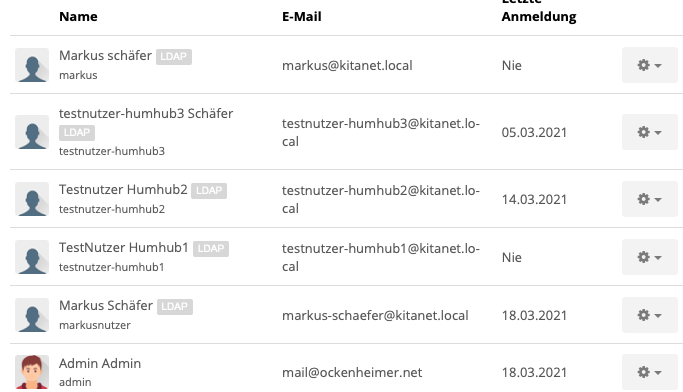
\includegraphics[width=1.0\textwidth]{res/nutzerliste.png}
  \caption{Nutzerliste der Testumgebung (Eigene Abbildung)}
  \label{fig:Nutzerliste}
\end{figure}

Das \ac{ldap} wird periodisch über einen sogenannten \textit{Cronjob} ausgelesen. Neue Nutzer werden entsprechend den oben dargestellten Kriterien angelegt und können sich ab diesem Moment mit dem in \ac{ldap} vergebenen Kennwort anmelden.

Dies schließt die Beschreibung des \textit{IST-Zustand} von Kitanet und der Testumgebung ab. Im folgenden werden nun die Grundlagen zum E-Mail-Versand dargestellt.

\chapter{Der Standard \textit{SMTP}}
\markboth{Der Standard \textit{SMTP}}{}
\label{sec:Der Standard}
Bereits in den Anfängen des \ac{arpanet} wurde die erste Software zum Versenden und Empfangen einer E-Mail zwischen Rechnern innerhalb eines Netzwerks entwickelt. \textquote{In March [1972] Ray Tomlinson at BBN wrote the basic email message send and read software, motivated by the need of the ARPAnet developers for an easy coordination mechanism. In July, Roberts expanded its utility by writing the first email utility program to list, selectively read, file, forward, and respond to messages. From there email took off as the largest network application for over a decade} \citep[][]{historyinternet}.

Hieraus entwickelte Jonathan Postel 1982 das \acf{smtp}.

Mit \ac{smtp} verband Postel den Wunsch, ein System zu schaffen, dass E-Mail unabhängig von der Transporttechnologie verlässlich und effizient transferiert \citep[vgl.][1]{rfc821}. Wie das Protokoll aufgebaut ist, wird nun anhand eines \textit{Gesprächs} zwischen zwei SMTP-Servern dargestellt und erläutert werden. Dieser Dialog wird in abgewandelter Form von Heinlein beschrieben \citep[vgl.][S. 24 ff.]{Heinlein2004}. 

\section{SMTP}

\textquote{The main purpose of SMTP is to deliver messages to user‘s mailboxes} \citep[][11]{rfc821}.
Wie von Postel formuliert, soll eine E-Mail via \ac{smtp} unabhängig vom Transportweg (\zb \ac{tcp}) von einem Nutzer versendet und vom Adressaten empfangen werden können. Sender ist in hier betrachtetem Dialog \verb+admin@kitanet+, Empfänger der E-Mail soll \verb+user@example.org+ sein. Den Datenaustausch vollziehen die SMTP-Server \verb+mail.kitanet+ als \textit{Client} und \verb+mail.example.org+ als \textit{Host}. Zur besseren Übersichtlichkeit werden Nachrichten des SMTP-Hosts mit H: eingeleitet, die des SMTP-Clients mit C:.

Das Design von \ac{smtp} sieht in seinem Kontext zwei Teilnehmer die Daten austauschen. Diese werden von ihm als \textit{Sender-SMTP} und \textit{Empfänger-SMTP} bezeichnet \citep[vgl.][2]{rfc821}. Dabei ist unabhängig, ob der Sender tatsächlich der Startpunkt für die Daten ist, oder ob der Empfänger der Endpunkt der Übertragung ist. Beide können auch nur Zwischenstationen innerhalb der Übertragung zwischen den Nutzern sein. \textquote{The receiver-SMTP may either be the ultimate destination or an intermediate} \citep[][2]{rfc821}.

Nach dem Herstellen der Verbindung meldet sich zunächst der Host:\\
\verb+H: Connected to mail.example.org+ \\ 
\verb+H: Escape Character ist '^]'+ \\
\verb+H: 220 mail.example.org SMTP Postfix on SuSE Linux 9.0 (i386)+

Der Host meldet mit Code 220 \textquote{Service ready} \citep[][38]{rfc821} dem Client, dass er zur Kommunikation bereit ist. 

Nun ist es am Client, sich zu identifizieren. \\
\verb+C: HELO mail.kitanet+ \\ 
\verb+H: 250 mail.example.org+

Mit Code 250 \textquote{Requested mail action okay, completed} \citep[][38]{rfc821} gibt der Host den Kommunikationskanal wieder frei.

Der Client meldet anschließend \\
\verb+C: MAIL FROM: <admin@kitanet>+ welches vom Host mit einem \\
\verb+H: 250 OK+ bestätigt wird.\\
Der Client verwendet den Befehl MAIL um die E-Mail-Transaktion zu starten. Er teilt dem Host mit, welchen Pfad das Datenpaket bisher genommen hat, bzw. welchen Weg eine eventuelle Antwort des Hosts nehmen muss um beim ursprünglichen Absender der Nachricht anzukommen. Postel spricht hier vom \textquote{reverse-path}. \textquote{When the list of hosts is present, it is a „reverse“ source route and indicates that the mail was relayed through each host on the list (the first host in the list was the most recent relay)}\citep[vgl.][20]{rfc821}.

Mit dem \ac{smtp}-Befehl\\
\verb+C: RCPT TO: <user@example.org>+ \\ 
und der Antwort des Hosts \\
\verb+H: 250 OK+\\
werden die einzelnen Empfänger der Mail gegenüber dem Host bekanntgegeben. Heinlein interpretiert die Antwort \verb+250 OK+ des Hosts damit, dass dieser sich für diese Nachricht \textquote{zuständig fühlt} \citep[vgl.][25]{Heinlein2004}.

Als nächstes folgt der Befehl \verb+DATA+. Die Antwort des Servers teilt dem Client zugleich mit, wie dieser anzeigen muss, wann der Datenblock übertragen wurde. Im Anschluss überträgt der Client die Nachricht und signalisiert das Ende der Daten mit dem Signal, in diesem Fall mit einem einzelnen Punkt.\\
\\
\verb+C: DATA+ \\
\verb+H: 354 End data with <CR><LF> . <CR><LF>+\\
\verb+C: Subject: Ein Betreff+ \\
\verb+C:+\\
\verb+C: Hallo Welt!+ \\
\verb+C:+\\ 
\verb+C:.+

Die Daten wurden nun vom Client an den Host übertragen. Dieser muss nun die Daten der Mail zur weiteren Verarbeitung vorbereiten und abspeichern. Als Antwort meldet er dem Client zurück, \textquote{unter welcher Kennung die E-Mail bei ihm erfolgreich gespeichert wurde} \citep[][25]{Heinlein2004}.\\
\verb+H: 250 Ok: queued as A6B701E890+ \\
Dies ist sogleich das Signal für den Client, die Mail aus seinem eigenen Speicher zu löschen, da Sie erfolgreich weitergeleitet wurde. Allerdings löscht er die Mail natürlich nur, wenn nicht die Mail nicht über einen anderen SMTP-Host an weitere Adressaten versendet werden muss.

Zum Beenden der Verbindung sendet der Client das Kommando \\
\verb+C: QUIT+, welches vom Host mit \\
\verb+H: 221 bye+ bestätigt wird. 

Hier war nur ein sehr vereinfachter Dialog zwischen Host und Client dargestellt. Postel stattete die Spezifikation mit weiteren, heute teils obsoleten, Optionen aus, wie z.B. der Möglichkeit Mails an ein Terminal zu verschicken, statt in ein Postfach \citep[vgl.][11]{rfc821} oder notwendigen Funktionalitäten wie dem Befehl EXPAND (EXPN) um die Teilnehmer einer Mailingliste anzeigen zu können \citep[vgl.][8]{rfc821}.

Auch musste der Host in der Lage sein, Verarbeitungsfehler mitzuteilen oder dem Client zu signalisieren, dass er den Empfänger nicht kannte. Der Umfang der gesamten Spezifikation würde hier den Rahmen sprengen, es sei insoweit auf \cite[][S. 37 ff.]{rfc821} verwiesen. Hier stellt Postel die möglichen Antworten für die SMTP-Kommandos dar.

Für die Kommunikation zwischen dem letzten SMTP-Server und dem \ac{mda} \citep[vgl.][28]{Heinlein2004} der die Mail letztendlich im lokalen Postfach ablegt, wurde das \ac{lmtp} entwickelt. \textquote{Es ist aber nicht dazu gedacht, SMTP/ESMTP zu ersetzen, es soll auch nicht gegenüber anderen Mailservern eingesetzt werden. Es soll allein für die lokale Kommunikation zum MDA eingesetzt werden und einen erheblichen Performancegewinn in Hochleistungsumgebungen bringen} \citep[][39]{Heinlein2004}. Im in dieser Bachelorarbeit eingesetzten Umfeld wird der  \ac{mda} vom IMAP-Client Dovecot bereitgestellt \citep[vgl.][]{dovecotlmtp}. Der \ac{smtp}-Server, der den Transport der Daten zwischen Sender und Empfänger verwaltet, wird auch als \ac{mta} bezeichnet \citep[vgl.][28]{Heinlein2004}.

SMTP in seiner Urform ist ein ASCII-basiertes System, also nur für die Weitergabe von Text spezifiziert. \textquote{The mail data may contain any of the 128 ASCII character codes}\citep[][21]{rfc821}. Entwicklungen wie \ac{mime} \citep[vgl.][]{rfc1521} lösten zwar das Problem der Datei-Anhänge, aber es entstand der Eindruck, der Veränderungs- und Erweiterungsdruck auf SMTP könnte die hohe Qualität des Standards gefährden. Man erkannte den Bedarf für einen Standard für Erweiterung von SMTP. So entstand der \ac{rfc} 1869.

\section{Enhanced SMTP}

1995 beschrieben Klensin u.a. im \ac{rfc} 1869 die \ac{esmtp}.
Sie wollten hierbei jedoch nicht einzelne Erweiterungen für SMTP beschreiben, sondern einen Rahmen schaffen, an den sich kommende SMTP-Erweiterungen orientieren können, aber auch müssen. \textquote{Rather than describing these extensions as separate and haphazard entities, this document enhances SMTP in an straightforward fashion that provides a framework in which all future extensions can be built in a single consistent way} \citep[][1]{rfc1869}. 

Gleichzeitig war es nicht ihre Absicht, es neuen Erweiterungen besonders einfach zu machen, SMTP als Unterbau zu verwenden. \textquote{This means that each and every extension, regardless of its benefits, must be carefully scrutinized [geprüft (Anm. d. Autors)] with respect to its implemetnation, deployment, and interoperability costs. In many cases, the cost of extending the SMTP serice will likely outweigh the benefit} \citep[][2]{rfc1869}. 

%\subsection{ESMTP-Framework}

Klensin u.a. führen in \ac{rfc} 1869 drei neue Faktoren in \ac{smtp} ein, um Erweiterungen des Standards zu vereinheitlichen.

\begin{itemize}
	\item{Den SMTP-Befehl \verb+EHLO+}\\
	Der Client, der \ac{esmtp} unterstützt soll den Dialog nicht mit dem Befehl \verb+HELO+, sondern mit \verb+EHLO+ (Extended HELO) einleiten, um damit zu prüfen, ob auch der SMTP-Host \ac{esmtp} unterstützt. Hierdurch ergab sich auch die Notwendigkeit, \ac{rfc} 821 zu erweitern, da als initialer Befehl nunmehr \verb+HELO+ und \verb+EHLO+ zugelassen sein mussten. Unterstützt der Host \ac{esmtp} nicht, sendet er auf den Befehl \verb+EHLO+ eine Fehlermeldung. Dies signalisiert dem Client, dass er mit dem Host nur ohne Erweiterungen sprechen kann \citep[vgl.][S. 3 ff.]{rfc1869}.
	\item{Zentrale Registrierung}\\
	Erweiterungen für \ac{esmtp} müssen zentral registriert und verwaltet werden. Hierfür sehen Klensin u.a. ein Zentralregister bei der \ac{iana} vor und schlagen zugleich die ersten Befehle vor \citep[vgl.][7]{rfc1869}. Hierbei handelt es sich um die von Postel 1982 vorgeschlagenen Befehle \verb+SEND+, \verb+SOML+, \verb+SAML+, \verb+EXPN+, \verb+HELP,+ und \verb+TURN+ \citep[für die Befehle vgl.][S. 23 ff.]{rfc821}.
	\item{erweiterte Parameter für \verb+MAIL FROM+ und \verb+RCPT TO+}\\
	Hier nehmen Klensin u.a. Bezug auf die bereits absehbaren Erweiterungen zu \ac{smtp}. \textquote{It is recognized that several of the extensions plannes for SMTP will make use of additional parameters associated with the MAIL FROM and RCPT TO command} \citep[][7]{rfc1869}. Im weiteren erläutern Sie die erforderliche Syntax für Befehle innerhalb von \verb+MAIL FROM+ und \verb+RCPT TO+ und betonen erneut die Notwendigkeit der Registrierung der Erweiterungen bei der \ac{iana}.
\end{itemize}

Durch die Erweiterungen und deren Registrierung entwickelte sich \ac{esmtp} zu einer sinnvollen Ergänzung. Dies mündete schließlich in der Übernahme des Systems in den Standard selbst \citep[vgl. u.a.][S. 7 ff]{rfc2821}.

Nachdem nun die theoretischen Grundlagen betrachtet wurden, werden im nächsten Kapitel die Anforderungen an den SMTP-Server im Rahmen des KitaNet formuliert. 





\chapter{Anforderungen an den SMTP-Server}
\markboth{Anforderungen an den SMTP-Server}{}
\label{sec:Anforderung}
Das Formulieren von Anforderungen zu Beginn eines Projektes ist, wie im Folgenden dargestellt, von entscheidender Bedeutung. \textquote{Requirement engineering is a technical process. Writing requirements is therefore not like other kinds of writing} \citep[][77]{Hull2010}. Zunächst wird nun die Theorie kurz erläutert, bevor anschließend diese Theorie auf das vorliegende Projekt angewandt und konkrete Anforderungen an die \ac{smtp}-Software formuliert werden.

\section{Theorie des Requirement Engineering}


Die Erwartungen eines Kunden zu einem fertigen Produkt werden zu lassen, ist die zentrale Aufgabe in der Entwicklung. Ein wichtiger Schritt steht hier bereits am Anfang des Projekts: Das Formulieren der Anforderungen.
\textquote{Die Anforderungen an ein neues Softwareprodukt zu ermitteln, zu spezifizieren, zu analysieren, zu validieren und daraus eine fachliche Lösung abzuleiten bzw. ein Produktmodell zu entwickeln, gehört mit zu den anspruchsvollsten Aufgaben innerhalb der Softwaretechnik} \citep[][434]{Balzert2010}. 
Balzert verwendet hierbei den, wie er ausführt, allgemein gebräuchlichen Begriff des \ac{re} \citep[vgl.][434]{Balzert2010}, der auch in dieser Arbeit Verwendung findet. Andere, in hier zitierten Publikationen verwendete synonyme Begriffe sind \zb das \textit{Anforderungsmanagement}.
\textquote{Anforderungen sorgen dafür, dass sowohl der Kunde als auch Ihre Organisation das Produkt bekommt, das sie wirklich wünschen und benötigen} \citep[][6]{Grande2014}.

\textquote{Erst die Anforderungen geben Ihrem Projekt das Fundament, um gezielt das Ist der Lösung mit dem Soll der Anforderungen zu vergleichen und auf diese Weise nachweisbar das Projektziel zu erfüllen} \citep[Fahney und Hermann in][10]{Herrmann2013}.
Fahney und Hermann beschreiben aber auch die Risiken schlecht formulierter Anforderungen. \textquote{Hat man ein Projekt begonnen, die Anforderungen jedoch unvollständig, widersprüchlich oder mehrdeutig erhoben, so läuft man Gefahr, das „falsche“ Projekt zu machen, selbst wenn man das Projekt „richtig“ macht} \citep[Fahney und Hermann in][10]{Herrmann2013}. 
Es bleibt somit festzuhalten, dass bereits die Anforderungen sorgsam behandelt werden müssen.

Laut Balters können Projekte einige Eigenschaften besitzen, die die Anforderungsermittlung beeinflussen. 
\blockquote{\textquote{Eine Vorgehensweise, um systematisch von der Anforderungsermittlung bis zum fertigen Produktmodell zu gelangen, hängt von vielen Randbedingungen ab:
	\begin{itemize}
		\item Liegt eine Ausschreibung vor, dann gibt es in der Regel bereits ein vom Auftraggeber erstelltes Lastenheft.
		\item Beauftragt eine Fachabteilung die interne IT-Abteilung mit der Softwareherstellung, dann gibt es außer Ideen der Fachabteilung vielleicht noch keine strukturierte schriftliche Unterlage.
		\item Gibt es bereits ein eingesetztes Softwaresystem, das abgelöst oder verbessert werden soll?
		\item Ist eine Individualsoftware zu entwickeln oder sind kundenspezifische Anpassungen an Standardsoftware vorzunehmen?
		\item Handelt es sich um eine innovative Softwareentwicklung, für die es keine Vorbilder gibt?
	\end{itemize}
Diese Rahmenbedingungen beeinflussen die Methodik} \citep[][435]{Balzert2010}.}

Einen Risikobereich für das \ac{re} wird von Dahm beschrieben. Dem Autor geht es hier um Probleme bei der Kommunikation mit dem Kunden. \textquote{Dabei wird häufig unterstellt, daß diese Kommunikation problemlos erfolgt, d.h., das durch die Kommunikation selbst keine Probleme erzeugt werden} \citep[][S. 174 f.]{Dahme2000}.
Der Autor führt dies anschließend weiter aus. 

	\blockquote{\textquote{So ist es meist falsch, anzunehmen, daß \\
	1. der Anwender bei Projektbeginn genau weiß, was er will, \\
 	2. der Anwender das, wovon er weiß, daß er es will, vollständig mitteilen kann, \\
 	3. der Entwickler ausreichend verstanden hat, was der Anwender mitteilen konnte,\\
 	4. das kommunizierte Wissen ausreicht, um die vom Anwender gewollten Funktionen produzieren zu können, \\
 	5. der Anwender versteht, was der Entwickler außer den vorgelegten Beispielen noch leisten könnte,\\
 	6. der Anwender wüßte, welche Software möglich wäre, wenn der Entwickler besser über seine Bedürfnisse unterrichtet wäre} \citep[][175]{Dahme2000}.}

Eine gute und genaue Kommunikation zwischen Kunden und Entwickler ist somit auch beim Festlegen der Anforderungen unerlässlich. 
Balzert bringt es auf den Punkt. 
\textquote{Anforderungen (\textit{requirements} [Hervorhebung im Original]) legen fest, was man von einem Softwaresystem als Eigenschaft erwartet} \citep[][455]{Balzert2010}.

Für die Formulierung von Anforderungen nennt Balzert neun Regeln. Sie sollen zunächst nach \cite[][S. 100 ff.]{Pohl2007} kurz und prägnant formuliert sein und den Akteur klar benennen. Darüber hinaus sollen die Anforderungen klar überprüfbare Ziele formulieren. Sofern dies nicht möglich ist, sollen die Ziele soweit verfeinert werden, dass die Teilziele überprüft werden können. \\
Es soll ferner beschrieben werden, welchen Nutzen das Ziel verfolgt, im Beispiel ist die Verkürzung der Bearbeitungszeit genannt. Durch die Begründung des Ziels soll die Identifikation weiterer Ziele erleichtert werden, jedoch soll bei der Formulierung kein Lösungsansatz angegeben werden. Des weiteren ergänzt Balzert nach \cite[][S. 100 f.]{Rupp2007}, dass es wichtig sei, einschränkende Rahmenbedingungen mit zu benennen und die Ziele realistisch zu formulieren \citep[vgl.][S. 457 ff.]{Balzert2010}.


Balzert beschreibt verschiedene Rahmenbedingungen, die die Auswahl und Entwicklung von Software beeinflussen. \textquote{Eine \textbf{Rahmenbedingung} \textit{(constraint)} [Hervorhebungen im Original]  - auch Restriktion genannt - legt organisatorische und/oder technische Restriktionen für das Softwaresystem und/oder den Entwicklungsprozess fest}\citep[][459]{Balzert2010}.
Hierunter zählen zum Einen \textit{organisatorische Rahmenbedingungen} wie der \textit{Anwendungsbereich} oder die \textit{Zielgruppe} für die eingesetzte Software. Auch \textit{Betriebsbedingungen}, wie die tägliche Nutzungszeit des Produktes oder ob das Produkt \zb für mobiles Arbeiten vorbereitet sein muss \citep[vgl.][S. 459 f.]{Balzert2010} gehören zu den organisatorischen Rahmenbedingungen. 
Zum Anderen nennt Balzert \textit{technische Rahmenbedingungen}, die eine Software erfüllen muss, um eingesetzt werden zu können. Diese sind die \textit{technische Produktumgebung}, also auf welcher Hardware und unter welchem Betriebssystem die Software funktionieren soll und die \textit{Anforderungen an die Entwicklungsumgebung}, in denen \ua festgelegt wird, welche Schnittstellen die Software bereitstellen muss oder welche Programmierumgebung verwendet werden muss \citep[vgl.][S. 460 f.]{Balzert2010}.

Weiteren Einfluss auf die Anforderungen nimmt der Nutzungskontext. Hierunter versteht Balzert die \textquote{materielle und immaterielle Umgebung} \citep[][461]{Balzert2010} in der das Softwaresystem zum Einsatz kommt. 
Unterschieden wird hier zwischen der für das System relevante Umgebung, den \textit{Kontext}, der bei der Systementwicklung zu betrachten sei, und der durch eine \textit{Grauzone} abgegrenzten irrelevanten Umgebung, wie in der folgenden Abbildung dargestellt \citep[vgl.][462]{Balzert2010}.

\begin{figure}[h]
  \centering
  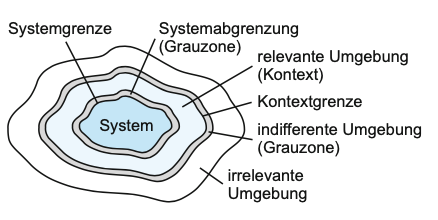
\includegraphics[width=0.8\textwidth]{res/Anforderung1.png}
  \caption{Das System und seine Umgebung \citep[][462]{Balzert2010})}
  \label{fig:Systemumgebung}
\end{figure}

Bisher wurden nur die \textit{funktionalen Anforderungen} beschrieben. Was soll das Produkt am Ende leisten, aus welchem Grund wird es entwickelt? Daneben gibt es eine weitere Art, nämlich die \textit{nichtfunktionalen Anforderungen}. \\ \textquote{\textbf{Nicht-funktionale Anforderungen} [Hervorhebung im Original] lassen sich qualitativ unterscheiden in \\
- Qualitätsattribute der gewünschten Funktionen \\ 
- Anforderungen an das implementierte System als Ganzes, \\ 
- Vorgaben für die Durchführung des Systemerstellung \\ 
- Anforderungen an Prüfung, Einführung, Betreuung und Betrieb} \citep[][S. 27 f.]{Partsch2010}.
Hierunter fallen somit sämtliche Aspekte, die nicht direkt einer Anforderung zuzuordnen sind, sondern das Produkt als ganzes betreffen \citep[vgl.][463]{Balzert2010}. Balzert nennt in diesem Zusammenhang \textquote{\ua Genauigkeit, Verfügbarkeit, Nebenläufigkeit, Konsumierbarkeit (eine Obermenge der Benutzbarkeit),[...], Zuverlässigkeit, Sicherheit, Service-Anforderungen, Support [...]} \citep[][463]{Balzert2010}. 
Partsch gibt im weiteren zu Bedenken, dass nichtfunktionale Anforderungen zumeist \textquote{wenn überhaupt, dann meist nicht präzise formuliert [werden]} \citep[][30]{Partsch2010}. Er begründet dies mit der Aussage bezüglich der Anforderung \textquote{(„Das weiß man ja“)} \citep[][30]{Partsch2010}.

Während die funktionalen Anforderungen beschreiben \textit{was} ein Produkt leisten muss, beschreiben nicht-funktionale Anforderungen \textit{wie} diese Leistung erbracht werden soll \citep[vgl.][30]{Partsch2010}.



\section{Anforderungsdokument nach dem IEEE}
Das \ac{ieee} ist eine der Institutionen, die sich mit der Standardisierung technischer Vorgänge beschäftigen. Ähnlich den bereits erwähnten \ac{rfc}, die unter der Schirmherrschaft der \ac{ietf} verwaltet werden, gibt das \ac{ieee} Standardisierungsvorschriften heraus. Eine dieser Schriften, die \ac{ieee} Std 830-1998, beschreibt die empfohlene Vorgehensweise bei der Spezifikation von Software Anforderungen (\ac{srs}).

Das \ac{ieee} gibt seinen Mitgliedern neben den Vorschriften auch ein Muster für \ac{srs} an die Hand. Da im Rahmen dieser Arbeit ebenfalls ein solches Anforderungsdokument erstellt wird, wird der Inhalt nun kurz erläutert \citep[vgl.][S. 11 ff.]{ieee1998}.
\begin{itemize}
	\item Einführung \citep[vgl.][S. 11 - 12]{ieee1998}
	\begin{itemize}
		\item Zweck des Dokuments \\
		Beschreibt den Grund, weshalb das Anforderungsdokument erstellt wird und an welche Zielgruppe sich das Dokument richtet.
		\item Umfang \\
		Beschreibt das Softwareprodukt und seinen Einsatzzweck. Wenn nötig beschreibt es auch, wofür das Produkt nicht gedacht ist. Hier werden erwartete Vorteile und Ziele des Projektes beschrieben.
		\item Definitionen, Akronyme, Abkürzungen \\
		Erläutert nicht geläufige Abkürzungen und Akronyme, liefert Definitionen soweit im allgemeinen Sprachgebrauch notwendig.
		\item Referenzen \\
		Verweist auf weiterführende Dokumentationen, die innerhalb des Anforderungsdokuments referenziert werden.
		\item Übersicht \\
		Erläutert, was das Dokument außer dem vorher genannten beinhaltet, sowie die Organisation innerhalb des Dokuments.
	\end{itemize}
	\item Produktübersicht \citep[vgl.][S. 12 - 15]{ieee1998}
	\begin{itemize}
		\item Produktperspektive \\
		Beschreibt das Produkt innerhalb der eingesetzten Umgebung und zeigt auf, wie es mit ihr interagiert, \zb verschiedene \textit{Interfaces} zur Nutzung von Hardware oder anderer Software.
		\item Produktfunktionen \\
		Beschreibt die Hauptfunktionen der Software
		\item Nutzereigenschaften \\
		Beschreibt, welcher Nutzer mit der Software interagiert. Hierbei wird der Schwerpunkt auf die Qualifikation, Schulung und Fortbildung des Nutzers gelegt.
		\item Einschränkungen \\
		Soll jegliche Einschränkungen erläutern, die das Produkt in seiner Umgebung beachten muss.
		\item Annahmen und Abhängigkeiten \\
		Beschreibt die Faktoren, die sich auf die Erstellung des Anforderungsdokuments ausgewirkt haben.
		\item verzögerte Anforderungen \\
		Beschreibt Anforderungen, die erst in der Zukunft realisiert werden können oder sollen.
	\end{itemize}
	\item Spezifische Funktionen \citep[vgl.][S. 15 - 20]{ieee1998}\\
	geht so detailliert auf Anforderungen ein, dass ein Systemdesigner das System entsprechend auf die Anforderung vorbereiten kann und ein Tester dies auch bestätigen kann. Jede Anforderung sollte zumindest eine Beschreibung jedes \textit{Inputs} und jedes damit in Zusammenhang stehenden \textit{Outputs} des Systems enthalten. Dieser Unterpunkt hängt stark von der Art des jeweiligen Produktes ab. Daher werden im Anhang des Standards mehrere Vorlagen für unterschiedliche Einsatzzwecke bereitgestellt. Ohne hier genauer auf die einzelnen Unterarten einzugehen, entscheidet sich der Autor für die Vorlage im Anhang 5, die die Anforderung nach \textit{Feature} unterteilt \citep[vgl.][23]{ieee1998}. Die einzelnen Unterpunkte sind:
	\begin{itemize}
		\item externe Schnittstellen \\
		detaillierte Beschreibung der Ein- und Ausgabe-Schnittstellen des Produkts (Es soll die Produktübersicht ergänzen, ohne sie unnötig zu wiederholen). Unterteilt werden sie in:
		\begin{itemize}
			\item Benutzerschnittstellen
			\item Hardwareschnittstellen
			\item Softwareschnittstellen
			\item Kommunikationsschnittstellen
		\end{itemize}
		\item Funktionen \\
		Hier werden die einzelnen Funktionen beschrieben. Der Standard gibt vor, die einzelnen Beschreibungen mit \textquote{The system shall...}(Das System soll... [Übersetzung des Autors]) \citep[][16]{ieee1998} einzuleiten.
		\begin{itemize}
			\item Funktion 1
			\begin{itemize}
				\item Zweck der Funktion
				\item Auslösung/Reaktion der Funktion \\
				Wie wird die spezifische Funktion ausgelöst, welches Ergebnis ist zu erwarten?
				\item Mit Funktion verbundene Anforderungen\\
				Welche Anforderung wird mit der Funktion erfüllt?
			\end{itemize}
			\item Funktion 2
			\item Funktion \textit{n}
		\end{itemize}
	\item Leistungsanforderung \\
	Beschreibt \zb wieviele gleichzeitige Anfragen das System verarbeiten muss.
	\item Design-Einschränkungen \\
	Beschreibt Einschränkungen die durch andere Standards oder Vorgaben des Unternehmens gegeben sind.
	\item Softwaresystem-Eigenschaften \\
	Beschreibt überprüfbare Parameter, um die Eignung der Software für den späteren Einsatzzweck zu verifizieren. Sie sind nochmal unterteilt in:
	\begin{itemize}
		\item Zuverlässigkeit 
		\item Verfügbarkeit
		\item Sicherheit
		\item Wartbarkeit
		\item Portierbarkeit
	\end{itemize} 
	\item andere Anforderungen \\
	Hier sind nicht funktionale Anforderungen beschrieben, die sich nicht unter die anderen Punkte einordnen ließen.
	\end{itemize}

\end{itemize}



In der Folge werden nun die erarbeiteten Grundlagen auf das vorliegende Projekt angewandt und die Anforderungen formuliert. 

\section{textliche Anforderungen}

\textquote{Bevor ein Softwaresystem entwickelt werden kann, muss festgestellt werden, welche Anforderungen es erfüllen soll} \citep[][454]{Balzert2010}.
Zunächst werden die Anforderungen im Freitext formuliert, bevor Sie anschließend in ein Anforderungsdokument überführt.  

Wie in Kapitel 2 beschrieben, arbeitet der Server mit dem Betriebssystem Ubuntu 20.04 LTS. Auf dem Server sind ferner ein \ac{ldap} installiert, dass die Informationen zu den Nutzern verwaltet. Das \ac{ldap} ist insoweit auch für den SMTP-Server von Bedeutung, da dieser Nutzern die Möglichkeit geben soll, sich beim SMTP-Server anzumelden um Mails zu versenden oder abzuholen. Der Abgleich und die Registrierung neuer Nutzer muss automatisch stattfinden.
Bereits entschieden wurde die Frage nach dem zu verwendenden Mail-Client. 
Da nicht abzusehen war, wie sich die technische Ausstattung der \ac{kita}, gerade in Hinsicht auf neu anzuschaffende Tablets, weiterentwickelt, sollte ein Webmail-Client verwendet werden, der keine zusätzlichen Ressourcen auf dem Endgerät verbraucht. Die Wahl fiel hier auf den \ac{imap}-Client \textit{Dovecot} \citep[vgl.][]{dovecotmain}. 

Wie Eingangs erwähnt befindet sich die \ac{kita} in Trägerschaft der Stadt Gau-Algesheim. Bereits bei der Anschaffung der Hardware für \textit{KitaNet} mussten die Studenten wert auf eine kostengünstige Anschaffung und geringe laufende Kosten legen. Auch bei der Auswahl der SMTP-Server-Software soll daher eine kostengünstige Lösung gefunden werden.

Technische Unterstützung erhält die  \ac{kita} grundsätzlich über die Verbandsgemeindeverwaltung Gau-Algesheim. Da die zwei dort beschäftigen Administratoren aber für alle Kindertagesstätten der Verbandsgemeinde zuständig sind, muss die Software wartungsarm angelegt sein. Im Störungsfall soll eine detaillierte Dokumentation die Fehlersuche vereinfachen.

Über das System sollen interne E-Mails ausgetauscht werden. Ein Mail-Verkehr mit dem Internet ist zunächst nicht geplant, sollte aber grundsätzlich möglich sein.
Da E-Mail ein asynchrones Kommunikationsmittel darstellt \citep[vgl.][10]{Duerscheid2003}, ist die Übertragungsgeschwindigkeit nach Meinung des Autors nicht von übermäßiger Bedeutung. Eine schnellere, als die Übertragungsdauer von 15 Stunden und 39 Minuten \citep[vgl.][]{maildauer}, die die \textit{erste deutsche E-Mail} von Laura Breeden an Michael Rotert erzielte, ist zu erwarten.

Aufgrund der oben genannten Anforderungen wurde ein Anforderungsdokument erstellt, wie vom \ac{ieee} vorgegeben (vgl. \autoref{ch:Anhang}). 

\section{Priorisierung}

Anforderungen an ein Produkt sind nie gleichwertig zueinander. 
\textquote{Some requirements are non-negotiable. If they are not met, the product is of no use} \citep[][83]{Hull2010}. Wie die Priorisierung der Anforderungen gestaltet werden kann, wird nun kurz dargestellt.

Hull u.a. schlagen vor, Anforderungen mit verschiedenen Werten auszustatten. Sie beschreiben in einem Beispiel die Werte M (mandatory limit), D (desired value) und B (best value) \citep[vgl.][83]{Hull2010}. \textquote{These three values can be held in separate attributes, or represented within the text in a labelled form, such as „The system shall support [M:50, D:100, B:200] simultaneous users“} \citep[][83]{Hull2010}.
Diese Methode gibt einzelnen Anforderungen eine gewisse Flexibilität, indem die Grenze für das Erreichen des Zieles klarer herausgestellt ist. Im genannten Beispiel sind 50 gleichzeitige Nutzer die Mindestgrenze, 100 Nutzer sind erstrebenswert, bestenfalls sind 200 gleichzeitige Nutzer möglich. Unterstützt die Lösung nun nur 99 Nutzer, \textquote{then it is most likely still of some value to the customer} \citep[][83]{Hull2010}.

Eine Aussage über die Wertigkeit der Anforderungen zueinander wird hier jedoch nicht getroffen. 

In besagtem Standard schlägt das \ac{ieee} vor, die Anforderungen nach ihrer Notwendigkeit einzuordnen. \textquote{Another way to rank requirements is to distinguish classes of requirements as essential, conditional, and optional} \citep[][7]{ieee1998}. Balzert steht dieser Einordnung kritisch gegenüber. \textquote{Erfahrungen haben gezeigt, dass die Verwendung dieser Ausprägungen dazu führt, dass die meisten Anforderungen mit \textbf{essenziel} [Hervorhebung im Original] gekennzeichnet werden, während optionale Anforderungen nur selten vorkommen} \citep[][543]{Balzert2010}.

Als Alternative schlägt Balzert die Verwendung des Kano-Modells vor. Dieses Modell bezieht sich auf die \textit{Theory of Attractive Quality} des japanischen Professors Noriaki Kano, dessen Studien einen Zusammenhang zwischen dem Erfüllen von Qualitätsmerkmalen einerseits und der Kundenzufriedenheit andererseits belegen \citep[vgl.][77]{Hoelzing2008}. \textquote{Durch eine Kundenbefragung im Rahmen einer Produktentwicklung werden nur geringfügige Mängel an den bisher angebotenen Modellen festgestellt. Daraus wird die Annahme abgeleitet, dass der Schlüssel zum Erfolg in eher latenten, nicht explizit artikulierten oder bewussten Kundenbedürfnissen liegt} \citep[][78]{Hoelzing2008}. Hölzing beschreibt im weitern wie Kano fünf Qualitätsattribute herausarbeitet \citep[vgl.][82]{Hoelzing2008}. Drei dieser fünf Eigenschaften bespricht dann auch Balzert.
\textquote{Die Produkteigenschaften werden in Kategorien eingeteilt:\\
- \textbf{Basiseigenschaften:} Vom Kunden selbstverständlich vorausgesetzte Eigenschaften (implizite Erwartung). Fehlt eine Basiseigenschaft, dann entsteht Unzufriedenheit. Werden sie erfüllt, dann entsteht aber \textit{keine} Zufriedenheit. \\
- \textbf{Leistungseigenschaften:} Vom Kunden bewusst geforderte Eigenschaften (Sonderausstattung!). Sie schaffen beim Kunden Zufriedenheit bzw. beseitigen Unzufriedenheit - je nach Ausmaß. \\
- \textbf{Begeisterungseigenschaften:} Eigenschaften die der Kunde \textit{nicht} erwartet hat. Die Kundenzufriedenheit wächst überproportional, wenn die Eigenschaft vorhanden ist [alle Hervorhebungen im Original]} \citep[][544]{Balzert2010}.
Übersetzt auf die Vorgaben des \ac{ieee}, entsprächen \textit{essential} somit \textit{Basiseigenschaften}, \textit{conditionell} wären mit den \textit{Leistungseigenschaften} gleichzusetzen und \textit{optional} bilden das Äquivalent zu \textit{Begeisterungseigenschaften}.

Die nicht durch Balzert benannten Eigenschaften sind von Hölzing nach Kano beschrieben. Es handelt sich um \textit{indifferent quality elements}, also Eigenschaften des Produktes, die weder Zufriedenheit noch Unzufriedenheit beim Kunden auslösen, sowie \textit{reverse quality elements}, welche eine höhere Zufriedenheit beim Kunden auslösen, je schlechter sie die Erwartungen des Kunden erfüllen \citep[vgl.][83]{Hoelzing2008}.

Das Verhältnis der Kundenzufriedenheit im Verhältnis zum Erfüllungsgrad der jeweiligen Produkteigenschaft ist in der folgenden Grafik visualisiert.

\begin{figure}[H]
  \centering
  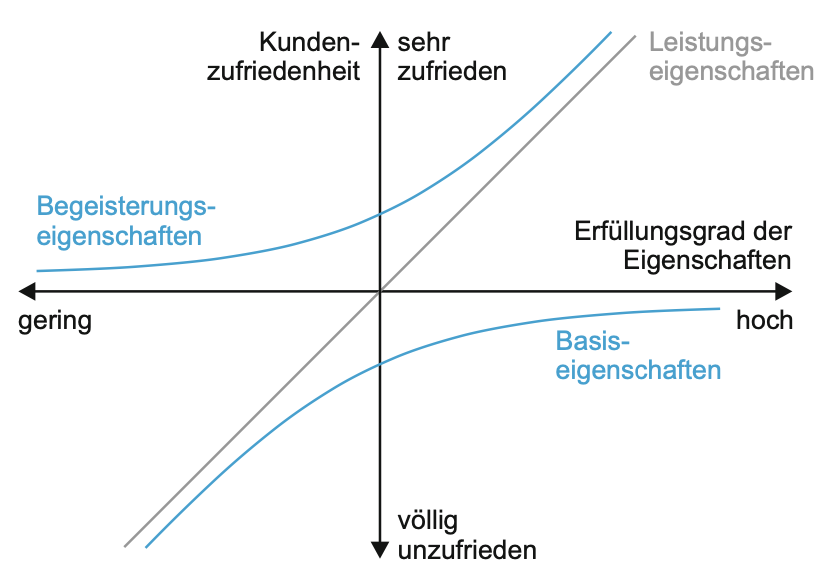
\includegraphics[width=0.6\textwidth]{res/kano.png}
  \caption{Die Entwicklung der Kundenzufriedenheit im Kano-Modell \citep[][545]{Balzert2010})}
  \label{fig:Kanomodell}
\end{figure}

Es wurden nun verschiedene Ansätze der Priorisierung und Wertung von Anforderungen besprochen. Der Autor dieser Bachelorarbeit ist im Rahmen seiner Tätigkeit bereits mit der Unterteilung der \ac{ieee} vertraut. Aus eigener Erfahrung kann er die Kritik von Balzert durchaus nachvollziehen, ist sich jedoch sicher, die Anforderungen sinnvoll abstufen zu können. Für die Priorisierung deren Anforderungen im Rahmen dieses Projekts sollen daher die Vorgaben der \ac{ieee} genutzt werden.

Gemäß der Definition innerhalb des Anforderungsdokuments (vgl. \autoref{ch:Definition}) sind folgende Anforderungen der ersten Priorität zuzuordnen:
\begin{itemize}
	\item (E)SMTP-Kommunikation
	\item Zusammenarbeit mit Dovecot
	\item Keine Anschaffungskosten
	\item keine Lizenzkosten
\end{itemize}

Das Anforderungsdokument bildet die Grundlage für die Entscheidung, welche Software für den \ac{smtp}-Server ausgewählt wird.

\section{Testformulierung}
\label{sec:test}

\textquote{Das Hauptziel des Freigabetestens ist, den Anbieter des Systems davon zu überzeugen, dass das System gut genug für die Benutzung ist} \citep[][266]{Sommerville2012}. 
Diese können je nach Projekt und Auftrag unterschiedlich ausgestaltet werden.  

Kleuker umschreibt einen Testfall als das simple Ausprobieren von Software \citep[vgl.][26]{Kleuker2019}. 
\textquote{Möchte man dies präzisieren, kommt man darauf, dass man drei Teilschritte erfassen muss: die Vorbedingungen, die Ausführung und die Nachbedingungen} \citep[][26]{Kleuker2019}.

Eine Form der Formulierung von Tests ist das anforderungsbasierte Testen.
\textquote{Bei anforderungsbasiertem Testen handelt es sich [...] um eine systematische Herangehensweise an den Testentwurf, in der Sie jede Anforderung in Betracht ziehen und eine Testreihe für sie gestalten} \citep[][266]{Sommerville2012}.
Sommerville gibt im weiteren zu Bedenken, dass zum Testen einer Anforderung unter Umständen ein einzelner Test ungenügend ist und verweist auch auf die Notwendigkeit Aufzeichnungen über die Tests zu führen \citep[vgl.][27]{Kleuker2019}.

\textquote{Bei der Testbeschreibung empfiehlt es sich, den Standard-Geschäftsprozess ohne Störungen zuerst zu beschreiben. Dann kann man in der Testbeschreibung den Prozess variieren, aber immer nur ein Detail} \citep[][161]{Witte2019}. Aufgrund der im vorigen Abschnitt formulierten Anforderungen sind unter anderem folgende Geschäftsprozesse denkbar:
\begin{itemize}
	\item Eine E-Mail wird geschrieben\\
	Die Anforderung an die Software mit der höchsten Priorität ist das Versenden von E-Mails als Kernaufgabe des Systems. Der Test wird  in der Art abgewandelt, dass eine Mail an einen nicht existenten Nutzer versendet wird.
	\item Ein Nutzer wird neu aufgenommen\\
	Eine weitere Anforderung stellt die Zusammenarbeit mit dem bereits im System verankerten LDAP dar. Hier muss getestet werden, ob eine neuer Nutzer zeitnah und ohne Zutun eines Administrators als Mail-Empfänger verfügbar ist. Eine Abwandlung dieses Test stellt das Löschen dieses Nutzers dar.
	\item Das System wird neu gestartet \\
	Die Anforderung \textit{Zuverlässigkeit} formuliert die Forderung, dass das System nach einem Serverneustart automatisch wieder startet. Hier werden zwei Szenarien abgebildet, nämlich der kontrollierte Neustart und der Neustart nach Stromausfall.
\end{itemize}


Mit diesen Grundlagen wurden anhand der Anforderungen Tests für das System formuliert, die nach der Implementation durchgeführt werden. 
Wie von Witte gefordert, achtete der Autor darauf die Tests möglichst kleinteilig zu beschreiben \citep[vgl.][S. 162 f.]{Witte2019}. Es soll auch einem fremden Dritten möglich sein, die Tests im Nachhinein nachvollziehen zu können. 
Die Tests wurden im Anhang dieser Arbeit zusammen mit der Dokumentation der Testdurchführung beigefügt (vgl. \autoref{ch:Testfaelle}). Der Aufbau der einzelnen Testfälle orientierte sich ebenfalls an Witte \citep[vgl.][162]{Witte2019}.


\chapter{Zur Auswahl stehende SMTP-Software}
\markboth{Zur Auswahl stehende SMTP-Software}{}
\label{sec:Auswahl}
In diesem Kapitel werden nun die zur Auswahl stehenden Softwarelösungen mit dem Anforderungsdokument verglichen und ihre Unterschiede aufgezeigt. 

Beide Softwarelösungen wurden vom Autor ausgewählt, da es sich um SMTP-Serversoftware handelt. Somit wird die primäre Anforderung, die Kommunikation über und Verarbeitung von (E)SMTP-Befehlen als gegeben vorausgesetzt.

Unterscheidungskriterien bilden die aus den Anforderungen gebildeten Unterpunkte:
\begin{itemize}
	\item Lauffähigkeit auf Ubuntu
	\item LDAP-Anbindung
	\item Dovecot-Unterstützung
	\item Wartungsfreier Betrieb
	\item Ausführliche Dokumentation
	\item Portierbarkeit auf andere Plattform
	\item keine Anschaffungskosten
	\item keine Lizenzkosten
\end{itemize}

Zunächst wird nun die Software Postfix betrachtet. Hier werden auch die grundlegenden Begrifflichkeiten erläutert.

\section{Postfix}
Postfix ist ein SMTP-Server-Programm, dass 1997  von Wietse Venema bei IBM entwickelt wurde, um als Alternative für das weit verbreitete Programm \textit{sendmail} zu dienen \citep[vgl.][307]{Deimeke2019}.

Postfix ist in Linux-Distributionen weit verbreitet. \textquote{Nahezu jede ernstzunehmende Linux-Distribution bringt natürlich auch ein vorkonfiguriertes Postfix-Paket mit, das sich wie jede andere Software per Tastendruck fertig kompiliert installieren lässt} \citep[][53]{Heinlein2004}.

Auch für Ubuntu 20.04 gibt es ein entsprechendes Paket. Tatsächlich stellt Postfix den Standard-\ac{mta} auf der Plattform dar \citep[vgl.][]{ubuntupostfix}.
Installationsanleitungen und Hilfe zu den Einstellungen der Software sind über das Wiki der Community verfügbar \citep[vgl.][]{ubuntupostfixwiki}. 

\textquote{There is also a Debian Wiki Postfix page that’s a bit more up to date; they also have a set of Postfix Tutorials for different Debian versions} \citep[][]{ubuntupostfix}. Da Ubuntu von dem Betriebssystem \textit{Debian} abgeleitet ist, können auch Beiträge im Debian-Wiki genutzt werden \citep[vgl.][]{debianpostfix}. 

Postfix ist LDAP-fähig.
Eine Anleitung zur Anbindung von Postfix an ein bestehendes LDAP findet sich beispielsweise in der in dieser Arbeit verwendeten Fachliteratur bei \cite[S. 689 ff.]{Deimeke2019} oder \cite[S. 106 f.]{Heinlein2004}. Aber auch im Wiki von Ubuntu gibt es eine, wenn auch nicht mehr ganz aktuelle, Anleitung zu diesem Thema \citep[vgl.][]{ubuntudovecotLDAPwiki}.

Auch Dovecot ist für die Zusammenarbeit mit Postfix vorbereitet. 
Gemäß Deimeke handelt es sich bei Dovecot um den \textquote{Shooting-Star unter den IMAP-Server: In den letzten Jahren hat er sich vom späten Newcomer zum technologisch führenden IMAP-Server entwickelt. Mächtig, robust, übersichtlich, logisch: Dovecot ist Admins Liebling} \citep[][338]{Deimeke2019}. 
So nimmt auch die Dokumentation von Dovecot regelmäßig Bezug auf Postfix \citep[vgl. z.B.][]{DovecotPostfix}.

Die Dokumentation von Postfix ist öffentlich einsehbar \citep[vgl.][]{postfixdoku}. Leider ist nicht ersichtlich, wie gut die umfangreiche Dokumentation gepflegt wurde, das einzige auffindbare Datum befand sich im Abschnitt \textit{Work in Progress} und gab das letzte Update mit \textquote{November 2013} an \citep[vgl.][]{postfixwip}. Jedoch wird die Software permanent weiterentwickelt. \\
Zum Zeitpunkt der Erstellung dieser Arbeit trägt der \textit{stable release} von Postfix die Versionsnummer 3.5.10, der \textit{Postfix 3.6 experimental release} wurde zuletzt mit am 11.04.2021 aktualisiert \citep[vgl.][]{postfixsource}. \\
Dass die Dokumentation dennoch dauerhaft gepflegt wird schließt der Autor beispielsweise aus der Tatsache, dass die im \textit{changelog} zu Version 3.5 angekündigte Unterstützung für mehrere \textit{relayhosts} \citep[vgl.][]{postfixcl35} im entsprechenden Abschnitt der Dokumentation vermerkt sind \citep[vgl.][]{postfixrelayhost}.

\textquote{Unter Portierung versteht man das Übertragen [eines Programms] auf ein anderes System} \citep[][26]{Habelitz2016}.
Habelitz führt weiter aus, dass der \textit{Quellcode} der Software für den Prozessor bzw. das entsprechende Betriebssystem kompiliert werden muss \citep[vgl.][27]{Habelitz2016}. 
Ist dieser Quellcode nicht verfügbar, kann das Programm nur auf den Betriebssystemen eingesetzt werden, die der Entwickler vorgesehen hat. 
Der Quellcode für Postfix ist öffentlich verfügbar \citep[vgl.][]{postfixsource}. 
Soweit dies durch die Lizenz der Software abgedeckt ist, in diesem Fall die \ac{epl} und \ac{ipl} \citep[vgl.][]{postfixsource}, kann diese in der Programmiersprache \textit{C} geschriebene Software auf jedem Betriebssystem eingesetzt werden, das C-Programme ausführen kann.
\textquote{C-Code kann portabel d. h. maschinenunabhängig sein. Er stimmt dann streng mit dem Standard überein (engl. \textbf{strictly conforming program} [Hervorhebung im Original])} \citep[][6]{Goll2014}. Im weiteren Verlauf geht Goll auch darauf ein, dass C auch maschinenspezifischen Code zulässt, der somit nicht portierbar sei. Der Autor sieht diesen Umstand jedoch im vorliegenden Fall für irrelevant, da Postfix bereits auf die meisten Server-Betriebssystemen portiert wurde \citep[vgl.][]{postfixpackages}.

Postfix steht wie bereits erwähnt unter der \ac{epl} und \ac{ipl}. Diese Open-Source-Lizenzen erlauben die kostenfreie private und kommerzielle Nutzung \citep[vgl.][]{postfixlizenz}. Somit fallen beim Einsatz von Postfix, wie gefordert, keine zusätzlichen Kosten an.

Nach der Betrachtung von Postfix werden nun die Eigenschaften von Exim untersucht.

\section{Exim}

\textquote{Exim is a message transfer agent (MTA) developed at the University of Cambridge for use on Unix systems connected to the Internet} \citep[][]{eximhome}. Die ursprünglich von Philip Hazel entwickelte Serversoftware sich, wie auch Postfix, als Ersatz für das Programm \textit{sendmail} \citep[vgl.][]{eximhome}. Sie bildet den Standard-\ac{mta} unter dem Betriebssystem \textit{Debian GNU/Linux}. \textquote{Exim generally comes with default Debian installation} \citep[][]{debianwiki}. Die Software liegt zur Erstellung dieser Bachelorarbeit in Version 4.94 vor \citep[vgl.][]{eximgit}.

Die Installationsanleitung und Einrichtungsdokumentation für Exim auf Ubuntu ist deutlich kleiner als für das bereits vorgestellte Postfix \citep[vgl.][]{eximubuntu}. \textquote{Exim4 can be installed in place of sendmail or Postfix [...]} \citep[][]{eximubuntu}. 

Insgesamt gestaltet sich die Recherche zu Exim schwierig, da auch die Entwickler keinen zentralen Anlaufpunkt pflegen. Die Dokumentation ist auf der offiziellen Homepage zu finden \citep[vgl.][]{eximdoku}, das Wiki und die Entwicklergemeinschaft werden aber auf der Softwareplattform \textit{github} verwaltet \citep[vgl.][]{eximwiki}. 

In den Dokumentationen ist der Umgang mit LDAP vermerkt. Die Autoren gehen hier auf die Unterschiede verschiedener LDAP-Implementationen ein und welche Auswirkungen dies auf die Einrichtung mit Exim mit sich bringt. \textquote{Unfortunately, though these are all compatible at the lookup function level, their error handling is different} \citep[][14.]{eximldap}. Auch die in dieser Arbeit verwendete Version \textit{OpenLDAP} wird unterstützt \citep[vgl.][14.]{eximldap}.

Auch die Konfiguration zur Verbindung mit Dovecot findet sich in der Dokumentation \citep[vgl.][]{eximdovecot}. Die Unterstützung des \ac{imap}-Servers ist somit gegeben.

Die Möglichkeiten zur Portierung der Software sind gegeben. Die Entwickler stellen Installationsanleitungen und -pakete für mehrere Linux-Betriebssysteme wie \textit{Suse-Linux}, \textit{Fedora} oder \textit{FreeBSD} \citep[vgl.][]{eximinstall}. 
Auch ist der Quelltext offen verfügbar, was für das in \textit{C} geschriebene Programm, wie bereits bei Postfix erwähnt, keinen nennenswerten Einschränkungen mit sich bringt \citep[vgl.][]{eximgit}. 

Im Gegensatz zu Postfix steht Exim unter der \ac{gpl} \citep[vgl.][]{eximhome}. Gemäß der \ac{gpl} darf der Entwickler \textquote{für jede übertragene Kopie [des Quellcodes] ein Entgelt - oder auch kein Entgelt - verlangen [...]} \citep[][4. Unveränderte Kopien]{gpldeutsch}. Im vorliegenden Fall ist das Projekt frei verfügbar. \textquote{It is freely available under the terms of the GNU General Public Licence} \citep[][]{eximhome}.
Somit fallen auch für diese Software zunächst keine Anschaffungs- oder Lizenzkosten an. Zwar schließt die Lizenz dies für die Zukunft nicht eindeutig aus, der Autor erachtet diese Möglichkeit jedoch als nur theoretisch gegeben an. 

Nachdem nun beide Pakete vorgestellt wurden, wird nun die Entscheidung getroffen und begründet.

\chapter{Entscheidung}
\markboth{Entscheidung}{}
\label{sec:Entscheidung}

Die Auswahl einer Software für den Einsatz im beruflichen Umfeld hat eine hohe Tragweite. Trifft man die falsche Wahl, kann man sich auf Jahre hinweg Ärger und Mehrarbeit einhandeln, da der Support mehr Mühe macht, als die fehlende Recherche zu Beginn Zeit gespart hat.

Sowohl Exim als auch Postfix stellen jede für sich brauchbare Lösungen zur Implementation eines SMTP-Servers im Umfeld von KitaNet dar. 

Die Wahl des Autors fällt hier auf Postfix, da diese Software die bessere und detailliertere Dokumentation für das momentan eingesetzte Betriebssystem Ubuntu liefert. Ein Großteil der recherchierten Fachliteratur nimmt auch Bezug auf das Zusammenspiel von Postfix als \ac{smtp}- und Dovecot als \ac{imap}-Server.
Die Möglichkeiten der Recherche in der Dokumentation oder in den Foren von Ubuntu-Hersteller Canonical übersteigen den Support von Exim bei Weitem.

Eine Stichproben-Suche nach dem Suchbegriff \verb+exim+ auf der deutschsprachigen Supporthomepage \verb+Ubuntuusers.de+ brachte ca. 200 Treffer \citep[vgl.][]{googleexim}, während die Suche nach \verb+postfix+ ungefähr 1.240 Ergebnisse lieferte \citep[vgl.][]{googlepostfix}.
Somit fiel die Wahl nicht zuletzt auf Postfix, da gerade für die mit der Wartung beauftragten lokalen Administratoren deutschsprachige Hilfeseiten essenziell wichtig sind.

Im weiteren Verlauf wird nun Postfix auf dem System installiert und in den Verbund aus Kitanet, OpenLDAP und Dovecot eingebettet.

\chapter{Installation und Tests}
\markboth{Installation und Tests}{}

Die Installation und Einrichtung von Postfix, Dovecot und Roundcube brachte kleinere und größere Probleme zu Tage. 
So lief zum Beispiel die Installation von Roundcube nicht fehlerfrei, wenn der SMTP-Server keine Authentifikationsmöglichkeiten \citep[vgl. hierzu][]{rfc5248} bereitstellte. 
Dies führte zu einer vorher nicht geplanten Installation von \textit{Cyrus SASL}, einem Dienst der einen \ac{sasl} bereitstellt. 

Der Autor sah ursprünglich keine Notwendigkeit, Postfix gegen das Versenden von von Mails durch Unberechtigte abzusichern, da weder der Server noch das Netzwerk an sich vom Internet aus erreichbar sind. 
Somit wurde dieser Aspekt in der Planung nicht in Betracht gezogen. 
Die zusätzliche Installation und Implementation von Cyrus SASL verlief dann aber problemlos, was auch dem modularen Aufbau von Postfix zu verdanken ist \citep[zu Postfix und Cyrus SASL vgl][S. 210 ff.]{Heinlein2004}.

Der folgende Abschnitt stellt somit einen idealisierten Installations- und Konfigurationsablauf dar.

\section{Einrichtung und Anbindung SMTP an LDAP}

Die Installation der Umgebung begann mit der Umkonfiguration von OpenLDAP. \textquote{Wenn Sie eigene Attribute benötigen, sollten Sie immer eine eigene Objektklasse in einem eigenen Schema erzeugen} \citep[][615]{Deimeke2019}. 
Nach diversen Recherchen sah der Autor die Notwendigkeit zusätzliche Attribute benötigt, um den Speicherort für das Postfach oder zusätzlicher Mailadressen für den Nutzer zu hinterlegen. 
Fündig wurde der Autor bei dem \textit{postfix-book.schema} welches in einer früheren Ausgabe von \cite{Heinlein2004} näher besprochen wurde \citep[vgl.][]{pfschema}. Die Veröffentlichung stellt eine Kopie des Schemas dar, das Original ist zum Zeitpunkt der Erstellung dieser Bachelorarbeit nicht mehr öffentlich zugänglich.

Dieses Schema führt die objectClass \textit{PostfixBookMailAccount} ein die unter anderem auch die Attribute die Attribute \textit{uniqueIdentifier} und \textit{mailEnabled} (welche bereits im Kapitel 2 genutzt wurden) ein. Darüber hinaus bietet die objectClass weitere E-Mail bezogene Attribute wie \zb \textit{mailAlias}.  

Nachdem das Schema in OpenLDAP geladen ist, wurden unter der neu angelegten \ac{ou} \textit{services} Konten für die benötigten Dienste \textit{kitanet}, \textit{postfix}, \textit{dovecot}, \textit{saslauth} und \textit{roundcube} angelegt. 
Über diese Konten werden die Abfragen in OpenLDAP durch die jeweiligen Dienste durchgeführt. 

Angelegt wurde auch der Nutzer \textit{ldaptest1}. Die Attribute dieses Nutzers sind in \autoref{ldapabfrage} dargestellt.

Grundsätzlich wäre dies auch über den zentralen Account \textit{cn=admin,dc=kitanet} möglich gewesen. 
Jedoch sollte im Protokoll von OpenLDAP unterschieden werden können, welcher Dienst ggf. eine fehlerhafte Abfrage stellt. 
Auch würde ein durch eine Sicherheitslücke kompromittiertes Passwort nur das Pflegen eines Dienstes, aber nicht gleich der ganzen E-Mail-Infrastruktur nötig machen.

Das Softwarepaket Postfix wurde über den Befehl \verb+sudo+ \verb+apt+ \verb+install+ \verb+postfix+ \\ \verb+postfix-ldap+ \verb+postfix-pcre+ installiert. 

\textquote{Die Konfiguration von Postfix spielt sich in \textit{/etc/postfix} ab, namentlich in den beiden Dateien \textit{main.cf} und \textit{master.cf}} \citep[][308]{Deimeke2019}.
Hier werden grundlegende Einstellungen wie die Festlegung des Hostnamens vorgenommen(vgl. \autoref{postfix/main.cf} Z. 9).

Die Zeilen 31-41 regeln die Zustellung von E-Mails an die in LDAP hinterlegten Empfänger via Dovecot. Hierzu werden auch die o.g. Dateien \verb+virtual_ldap_recipients+ und \verb+virtual_ldap_aliases+ eingebunden (vgl. \autoref{postfix/main.cf} Z. 39-41).

Zeile 47 schaltet die Authentifikation nach \ac{rfc} 4954 frei.
In den Zeilen 49 ff. wird festgelegt, wie sich Postfix während einem SMTP-Dialog verhalten soll.
So lehnt Postfix \zb gemäß Z. 52 E-Mails ab, welche keinen \ac{fqdn} als Empfänger haben \citep[vgl.][]{postfixfqdn}. 
Der \ac{fqdn} des hier eingerichteten Mailserver \verb+mail.kitanet.local+ wäre \zb \verb+kitanet.local+ \citep[vgl.][]{fqdn}. 
Somit würde in diesem Beispiel eine E-Mail mit dem hypothetischen Empfänger \verb+test@kitanet+ nicht angenommen werden.

\autoref{postfix/recipients.cf} zeigt die Konfiguration für eine Abfrage im LDAP zur Ermittlung der Empfänger über die Datei \verb+virtual_ldap_recipients+.
Die LDAP-Abfrage aus Zeile 14 übergibt die Variable \%s (die Mailadresse des Empfängers) an OpenLDAP und erwartet das Attribut \verb+mail+ des entsprechenden Datenbank-Eintrags zurück, was mit der Eingabe übereinstimmen muss. Hierdurch stellt Postfix sicher, dass die Mail-Adresse einem Nutzer zugeordnet wurde. Die Abfrage nach einem nicht existenten Nutzer würde eine leere Antwort zurückgeben, ungleich zur Anfrage.

Wird der Empfänger nicht gefunden, prüft Postfix ob die Adresse als mailAlias bei einem Nutzer erfasst wurde. Hierzu dient die Datei \verb+virtual_ldap_aliases+ (vgl. \autoref{postfix/aliases.cf}). 
Diese Datei unterscheidet sich nur in dem abgefragten Attribut in Zeile 14. 
Hier wird das Attribut \textit{mailAlias} abgefragt. 
Im Beispiel von \autoref{ldapabfrage} würde eine Anfrage nach der Adresse \verb+postmaster@kitanet.local+ die \textit{primäre} Mail-Adresse des Empfängers, nämlich \verb+administrator@kitanet.local+ zurückgeben. 
Postfix kann dann die E-Mail in das korrekte Postfach ablegen.

Cyrus SASL wurde wie oben erläutert innerhalb des Systems installiert. 
Die Authentifizierung eines SMTP-Nutzers innerhalb von Postfix wird über die Datei\\\verb+/etc/postfix/sasl/smtpd.conf+ gesteuert (vgl. \autoref{postfix/sasl} Z. 2). 
Die Nutzer haben keinen Zugriff auf den Server, bzw. die Protokollierung innerhalb des Servers.
Daher hat der Autor keinen zusätzlichen Verschlüsselungsdienst eingerichtet. 
Die Passwörter werden daher unverschlüsselt (\verb+PLAIN LOGIN+) übermittelt (vgl. \autoref{postfix/sasl} Z. 3). 

Dovecot und Roundcube wurden ebenfalls entsprechend Dokumentation installiert. Auch sie greifen über eigene Nutzer auf LDAP zu um die Nutzer zu verwalten. Die Authentifikation wird ebenfalls über Cyrus SASL durchgeführt.

Nach Installation von Roundcube und Anmeldung eines bereits in Kitanet aktiven Nutzers wartete bereits die erste Mail auf den Autor.

\begin{figure}[H]
  \centering
  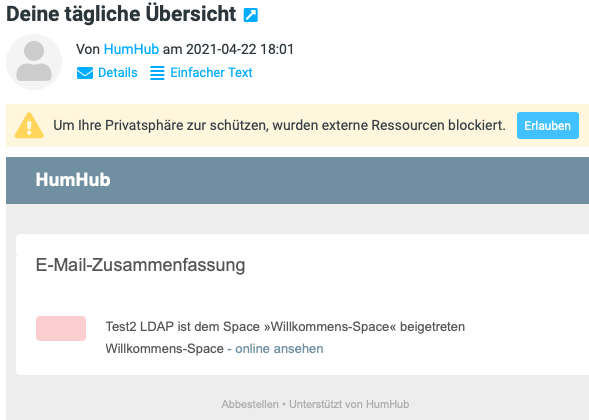
\includegraphics[width=0.72\textwidth]{res/erste Mail.png}
  \caption{Die erste E-Mail im Posteingang (Eigene Darstellung)}
  \label{fig:Mail}
\end{figure}

\section{Tests}{}
Nach der erfolgreichen Einrichtung und den ersten testweise und über die Kommandozeile versendeten E-Mails war es an der Zeit, die in \autoref{sec:test} formulierten Tests durchzuführen. Das Ergebnis der Tests ist bereits in \autoref{ch:Testfaelle} erfasst worden.
\subsection{Dokumentation der einzelnen Tests}
Wurde der Test bestanden? Musste der Test unerwartet an die Gegebenheiten angepasst werden?

\chapter{Fazit}
\markboth{Fazit}{}
\label{sec:Fazit}

\blindtext


